\chapter{A sample of Lean}
The following chapter provides a concise overview of the author's experience with lean, the challenges encountered, and the author's approach to formalisation. 

However, it will not explain the operational logic of lean nor serve as a guide to learning lean, as this is beyond the scope of this thesis.
 For those interested in learning more about lean, I recommend consulting the following resources: \url{https://leanprover-community.github.io/learn.html}

\section{Working with Lean}
\subsection*{Blueprint}
\begin{wrapfigure}{r}{0.5\textwidth}
    \centering
    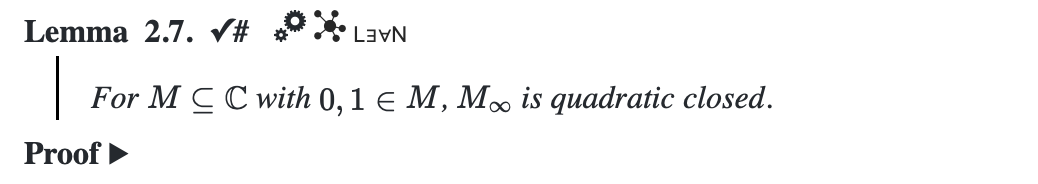
\includegraphics[angle=0, width=0.5\textwidth]{Blueprint}
    \label{fig:Blueprint}
    \caption{Blueprint}
    \scriptsize
    \begin{itemize}
        \setlength\itemsep{-0.5em}
        \item[$\checkmark$] Indicates the statment is Formalised
        \item[$\#$] Links to the proof
        \item[\scalebox{0.1}{
\includegraphics{gear}}] Shows to the proof
        \item[\scalebox{0.1}{
\includegraphics{mindmap}}] Shows dependency
        \item[\scalebox{0.5}{$\text{L}\exists\forall\text{N}$}] Links to the documentation
    \end{itemize}
\end{wrapfigure}

In order to structure my project, I employ the Lean Blueprint tool, created by Patrick Massot. \cite{Massot_2020}
This tool generates a web version of the LaTeX file, which provides an outline of the project and facilitates the integration of code with the associated documentation. 
Please refer to Figure \ref{fig:Blueprint} for an example of the linking. 
Furthermore, it generates a dependency graph \ref{fig:DependencyGraph}, which illustrates the extent of formalisation.
The presented approach is particularly beneficial for larger-scale projects involving multiple contributors, as evidenced in Terence Tao blog post. \cite{Tao_2023}



\subsection*{Lean}
Should i write about lean???
\clearpage
\begin{figure}[h]
    \centering
    \scalebox{0.5}{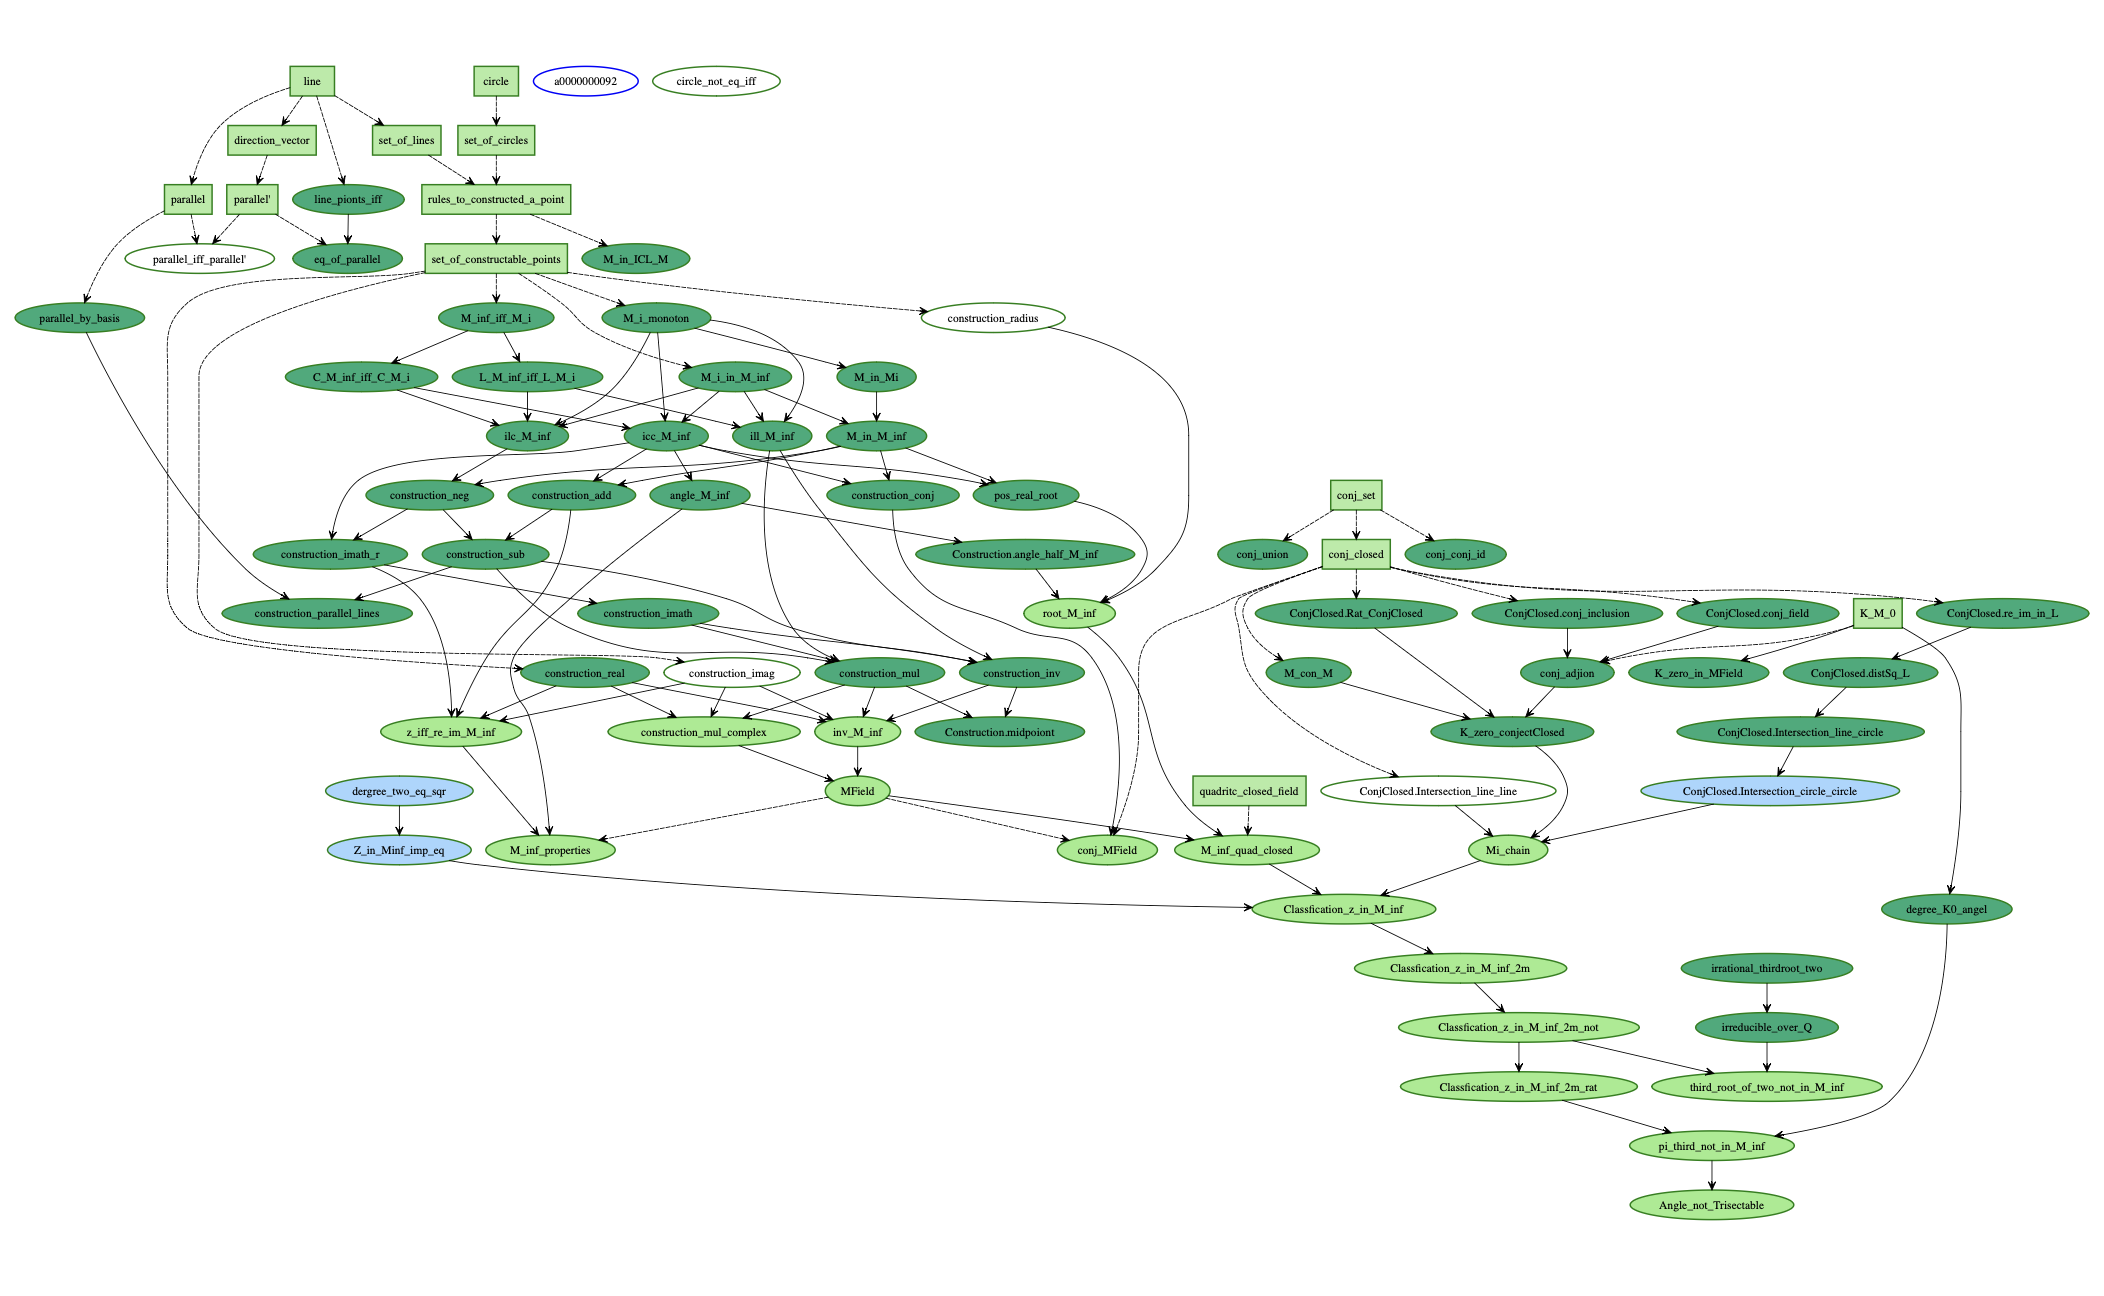
\includegraphics[angle=90]{DependencyGraph}}
    \label{fig:DependencyGraph}
    \caption{Dependency Graph}
\end{figure}
\clearpage
\section{A sample of Lean code} 
The following is a representative sample of the Lean code, which is available in its entirety on the GitHub repository of this project. 
\url{https://github.com/Louis-Le-Grand/Formalisation-of-constructable-numbers}

I defined lines as a structure of two points $z_1$ and $z_2$. 
For this structure I then define points by $\{\lambda z_1 + (1-\lambda)z_2\mid\lambda\in\R\}$ which are all the points the line goes through. 
I have omitted the condition $z_1\ne z_2$ because in some settings a line that consists of only one point makes sense.
\begin{lstlisting}
    structure line where
        (z₁ z₂ : ℂ)

    def line.points (l: line) : Set ℂ:= 
        {(t : ℂ) * l.z₁ + (1-t) * l.z₂ | (t : ℝ)}
\end{lstlisting}

To define the circles, I used $c$ of $\C$ as the centre and $r$ as the radius. 
For the points, I could refer to spheres already defined in Mathilb, which had the advantage that I could use existing lemmas about them. 
\begin{lstlisting}
    structure circle where
        (c : ℂ)
        (r : ℝ)

    def circle.points (c: circle) := Metric.sphere c.c c.r
    noncomputable def circle.points' (c: circle) := 
        (⟨c.c, c.r⟩ : EuclideanGeometry.Sphere ℂ)
\end{lstlisting}

To prove that $M_{\infty}$ is a subfile of $\C$, I had to define a new object of type subfile of $\C$, and use $M_{\infty}$ as the subordinate carrier.
This is because each object in Lean is a type, and you cannot switch between types.
\begin{lstlisting}
    noncomputable def MField (M: Set ℂ)(h₀: 0 ∈ M)(h₁: 1∈ M):
            Subfield ℂ where
        carrier := M_inf M
        zero_mem' := by exact M_M_inf M h₀
        one_mem' := by exact M_M_inf M h₁
        add_mem' := by apply add_M_Inf M h₀
        neg_mem' := by apply z_neg_M_inf M h₀
        mul_mem' := by apply mul_M_inf M h₀ h₁
        inv_mem' := by apply inv_M_inf M h₀ h₁
\end{lstlisting}
